%!TEX root = report.tex

\chapter{Experiments}
\label{chp:experiments}
In this chapter we detail the experiments performed on the model described in
\fullref{chp:theorystuff} and discuss the respective results.

\section{First experiment}

% documentazione wrapfig: https://ctan.mirror.garr.it/mirrors/ctan/macros/latex/contrib/wrapfig/wrapfig-doc.pdf
% lo segno perché il primo parametro opzionale può tornare utile
\begin{wrapfigure}[17]{r}{0.5\textwidth}
    \centering
    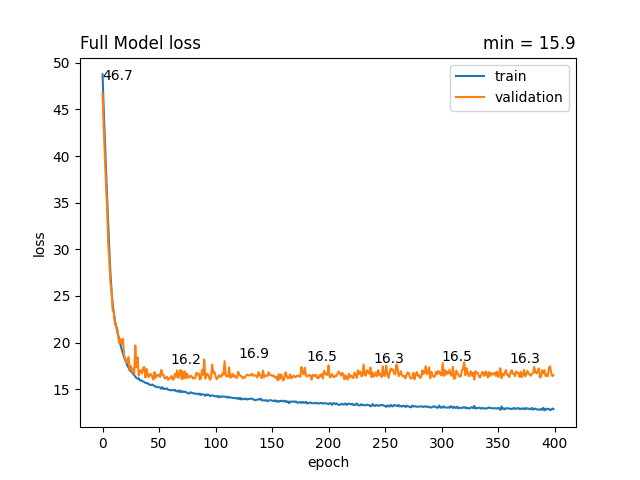
\includegraphics[width=0.5\textwidth]{400_loss}
    \caption{Initial experiment loss (400 epochs on Wiki)}
    \label{fig:400_loss}
\end{wrapfigure}

An initial experiment was performed by training the C3AE model for
400 epochs on the Wiki dataset as a means to test the \texttt{tensorflow} environment
and the functioning of the implemented C3AE model within it.

The evolution of training and validation loss is shown in \autoref{fig:400_loss}.
The experiment ran to completition with no runtime errors, and
it can be observed that the model was able to decrease its loss,
and that such loss reached an asymptote around epoch 50.

For this reason, we concluded that a training time of 400 epochs
is too much for this model and decided to set the epoch limit to 100 for
all following experiments, assuming that they would have a similar
evolution to this one and therefore all significant improvement
would happen much before the 100\textsuperscript{th} epoch,
in order to reduce the experiments' computation time.

\section{Performance evaluation over multiple datasets}

All the following experiments have been performed on datasets processed with the 
augmentation techniques described in \fullref{sec:augmentation} unless stated otherwise.

\subsection{Wiki}

\begin{wrapfigure}[17]{r}{0.5\textwidth}
  \centering
  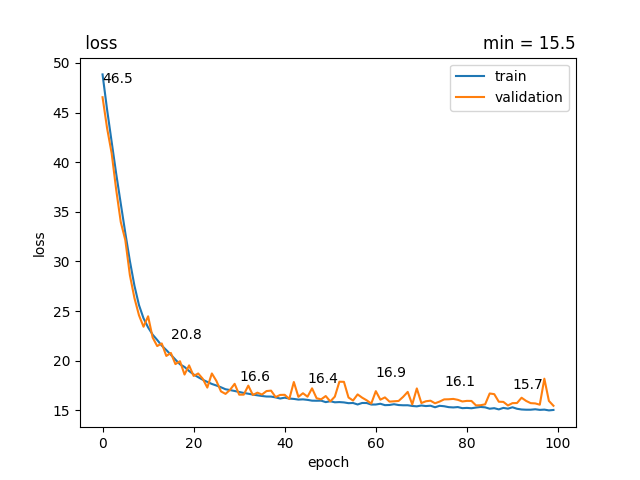
\includegraphics[width=0.5\textwidth]{full_model_loss}
  \caption{MAE on Wiki dataset (100 epochs)}
  \label{fig:wiki_loss}
\end{wrapfigure}

The first and main dataset used in our experiments has been Wiki.
As shown in the loss graph in \autoref{fig:wiki_loss} the learning curve is
correct and the best MAE value obtained in this experiment is 6.79 years. 
When compared to the result in the original paper, which claims to have reached 
a MAE of 6.44 on the same dataset, we could say that we have pretty much achieved
a state-of-the-art performance.

However, this result only takes in consideration Wiki images for both training
and validation. So we tested the output of this experiment with the FGNET test set,
and found a much higher MAE of 18.1 years.
The main reason for this is that the Wiki dataset is mostly composed by images
of adults and elders and features almost no children, while FGNET has a much lower
age on average and comprises even newborns with a declared age of 0 years. 
The result is that the model in this experiment always overshoots the age of the 
subjects and thus we obtain a high error.

\subsection{Utk}

\begin{wrapfigure}[17]{r}{0.5\textwidth}
  \centering
  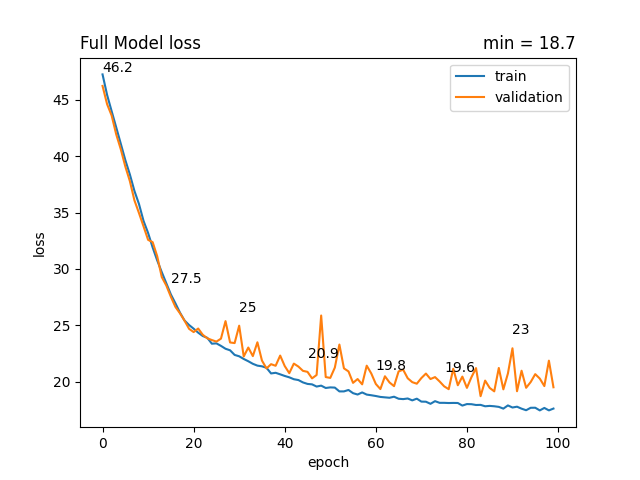
\includegraphics[width=0.5\textwidth]{utk_loss}
  \caption{MAE on UTK dataset (100 epochs)}
  \label{fig:utk_loss}
\end{wrapfigure}

In this experiment the starting conditions and parameters are the same as the 
previous one, but the dataset this time is UTK. The number of images is one third
of Wiki, but it covers better the whole range of ages from 0 to over 100.
As a matter of fact the validation MAE (computed on the UTK set itself) is slightly
higher than before at 8.67, but the test MAE on FGNET is almost halved, at 9.79 years.

The conclusion is that UTK is a better dataset for our experiments, but we can still 
use Wiki, as seen on the next experiment

\subsection{Wiki + Utk}
\label{sec:wikiutk}

\begin{wrapfigure}[17]{r}{0.5\textwidth}
  \centering
  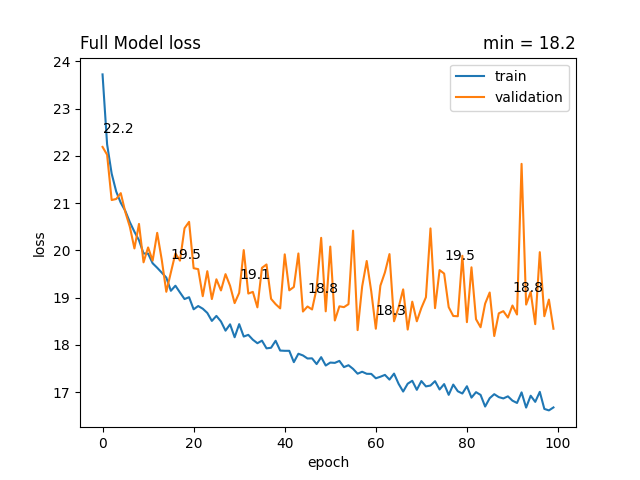
\includegraphics[width=0.5\textwidth]{wiki+utk_200_loss}
  \caption{MAE on Wiki+Utk dataset (100 epochs)}
  \label{fig:wiki+utk_loss}
\end{wrapfigure}

This third experiment combines the previous two. We started by pre-training a model from 
scratch with the Wiki dataset, and then we took the output of this process and further 
trained it for another 100 epochs on the UTK dataset. In this way we hoped to combine the
scale of the first dataset with the completeness of the second to obtain a model that
outperforms the previous two. And indeed, with a final validation MAE of 8.23 and a test
MAE of 8.64 years on FGNET this has proven to be our best result yet.

\section{Ablation Study}
\label{sec:ablation_study}
A separate set of experiments was performed to study the impact on performance
of the following components of the model and the training process:
the context module and the cascade module of the C3AE model,
and the training data augmentation.

We trained the following variants of the full C3AE model:

\begin{itemize}
  \item \textit{Full model}: the standard model with no changes,
    to serve as a benchmark against the other variants.
  \item \textit{No augmentation}: the data augmentation transformations
    on the training data are disabled.
  \item \textit{No context}: the context module of C3AE is excluded.
    Therefore, only one crop, the outermost one, is given as input to
    the model, and obviously there is no concatenation phase.
  \item \textit{No cascade}: the cascade module of C3AE is excluded.
    Consequently, the intermediate layer between the concatenated feature vector
    and the age output loses its meaning of two-point representation of age
    and becomes a plain hidden layer. This also means that this variant
    does not compute any KL Divergence and outputs only the final age estimation;
    the loss depends only on the age MAE as well.
  \item \textit{No context and no cascade}: both modules are disabled.
\end{itemize}

Each variant was trained for 100 epochs on the Wiki dataset.

((plot and discuss results))
